\chapter{الاحتراق: ما تحتاج إليه النار}\label{ch:g4:what-a-fire-needs}

نار مخيم عند الغسق. احتاجت إلى خشب جاف، وإلى عود ثقاب لإشعالها، والريح
التي تهب فيها تبقيها متوهجة. وبعد ساعة تكون الحطبات قد صارت جمرًا
متوهجًا ورمادًا أبيض، ويكون دخان رمادي قد ارتفع بعيدًا في السماء. فأين
ذهب الخشب؟ وماذا تحتاج النار، وماذا تترك وراءها؟

\begin{recall}
\omterm{def:g4:air-a-mixture-of-gases:air}{الهواء} خليط من الغازات: نحو أربعة أخماسه نيتروجين وخمسه أكسجين، ومعهما
قليل من الأرغون وثنائي أكسيد الكربون. واللهب يأخذ الأكسجين من \omterm{def:g4:air-a-mixture-of-gases:air}{الهواء}
المحيط به؛ والشمعة تحت الناقوس تنطفئ حين يبقى أكسجين قليل جدًا
(\cref{ch:g4:air-a-mixture-of-gases}).
\end{recall}

\begin{omfigure}
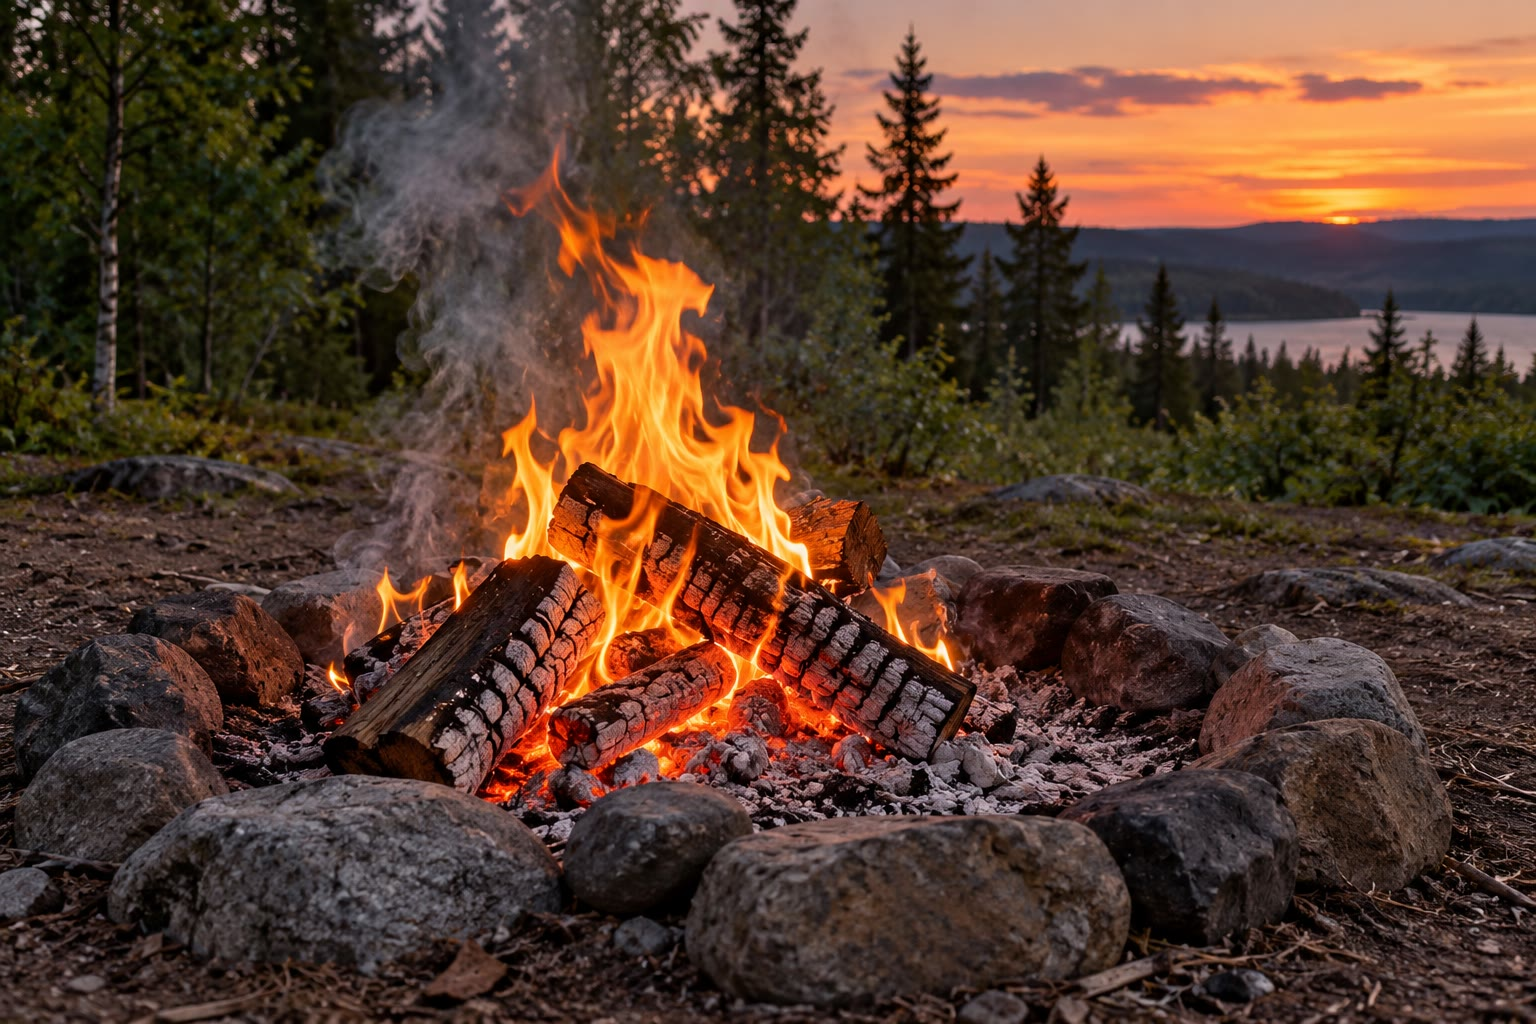
\includegraphics[width=0.6\linewidth]{images/book1/ai/g4-campfire.jpg}

{\small نار مخيم: خشب \omterm{def:g4:air-a-mixture-of-gases:air}{وهواء} وعود ثقاب --- وبعد ذلك رماد
ودخان.}
\end{omfigure}

\section{أنواع الوقود}

\begin{definition}[الوقود]\label{def:g4:what-a-fire-needs:fuel}
\emph{الوقود}\index{وقود} مادة يمكن أن تحترق فتُطلق حرارة وضوءًا:
الخشب، والورق، والفحم، وشمع الشموع، وغاز الموقد، والبنزين، وزيت
التدفئة.
\end{definition}

\begin{example}[وقود صلب وسائل وغازي]\label{ex:g4:what-a-fire-needs:fuels}
الخشب والورق والفحم وشمع الشموع أنواع \omterm{def:g4:what-a-fire-needs:fuel}{وقود} صلبة. والبنزين وزيت التدفئة
أنواع \omterm{def:g4:what-a-fire-needs:fuel}{وقود} سائلة. وغاز موقد المطبخ والغاز الذي في القداحة أنواع \omterm{def:g4:what-a-fire-needs:fuel}{وقود}
غازية.
\end{example}

\begin{remark}[ليس كل شيء يحترق]\label{rem:g4:what-a-fire-needs:not}
الحجر والرمل والزجاج والماء لا تحترق: فهي ليست وقودًا. ولهذا تُبنى
المدفأة من الحجر أو الطوب، ويُستعمل الرمل والماء لإطفاء
الحرائق.
\end{remark}

\section{مثلث النار}

\begin{definition}[مثلث النار]\label{def:g4:what-a-fire-needs:fire-triangle}
تحتاج النار إلى ثلاثة أشياء معًا: \omterm{def:g4:what-a-fire-needs:fuel}{وقود}، وأكسجين من \omterm{def:g4:air-a-mixture-of-gases:air}{الهواء}، وحرارة
لإشعالها. وتُرسم هذه الأشياء الثلاثة أضلاعًا ثلاثة لمثلث هو
\emph{مثلث النار}\index{مثلث النار}. فإذا غاب ضلع منها فلا
نار.
\end{definition}

\begin{omfigure}
\begin{tikzpicture}[font=\small]
  \coordinate (A) at (0,0); \coordinate (B) at (5,0); \coordinate (C) at (2.5,4.1);
  \draw[line width=3pt, brown!70!black] (A) -- (B);
  \draw[line width=3pt, omDef] (B) -- (C);
  \draw[line width=3pt, red!75!black] (C) -- (A);
  \node[below=4pt, font=\small\bfseries, brown!60!black] at (2.5,0) {الوقود};
  \node[right=4pt, font=\small\bfseries, omDef] at (3.75,2.05) {الأكسجين (من الهواء)};
  \node[left=4pt, font=\small\bfseries, red!75!black] at (1.25,2.05) {الحرارة (للإشعال)};
  % a flame in the middle
  \fill[orange!80] (2.5,0.55) .. controls (1.95,1.15) and (2.35,1.75) .. (2.55,2.3)
    .. controls (2.75,1.75) and (3.05,1.15) .. (2.5,0.55);
  \fill[yellow!80] (2.5,0.7) .. controls (2.25,1.05) and (2.4,1.35) .. (2.52,1.65)
    .. controls (2.62,1.35) and (2.75,1.05) .. (2.5,0.7);
\end{tikzpicture}

{\small \omterm{def:g4:what-a-fire-needs:fire-triangle}{مثلث النار}: \omterm{def:g4:what-a-fire-needs:fuel}{الوقود} والأكسجين والحرارة، الثلاثة معًا.}
\end{omfigure}

\begin{example}[إشعال عود ثقاب]\label{ex:g4:what-a-fire-needs:match}
نحك رأس عود الثقاب بجانب علبته. فيسخّنه الحك بما يكفي ليبدأ في
\omterm{def:g4:what-a-fire-needs:burning}{الاحتراق}: هذا ضلع الحرارة في المثلث. وخشب العود هو \omterm{def:g4:what-a-fire-needs:fuel}{الوقود}، \omterm{def:g4:air-a-mixture-of-gases:air}{والهواء}
يأتي بالأكسجين.
\end{example}

\begin{example}[النفخ على الجمر]\label{ex:g4:what-a-fire-needs:embers}
الجمر المتوهج الذي يبدو كأنه يكاد ينطفئ يشتعل لهبًا من جديد حين ينفخ عليه
أحد: فالنفخ يأتي \omterm{def:g4:air-a-mixture-of-gases:air}{بهواء} أكثر، وبالتالي بأكسجين أكثر، إلى \omterm{def:g4:what-a-fire-needs:fuel}{الوقود} الذي لا
يزال ساخنًا.
\end{example}

\section{الاحتراق يُنتج مواد جديدة}

\begin{definition}[الاشتعال والاحتراق]\label{def:g4:what-a-fire-needs:burning}
\emph{الاشتعال}\index{اشتعال} هو ما يحدث حين يأخذ \omterm{def:g4:what-a-fire-needs:fuel}{الوقود} الأكسجين من
\omterm{def:g4:air-a-mixture-of-gases:air}{الهواء} ويُطلق حرارة وضوءًا. ويسمي الكيميائيون الاشتعال
\emph{احتراقًا}\index{احتراق}. وفي أثناء الاحتراق يُستهلك \omterm{def:g4:what-a-fire-needs:fuel}{الوقود}
والأكسجين، وتظهر مواد جديدة: الدخان، والرماد، وثنائي أكسيد الكربون،
وبخار الماء.
\end{definition}

\begin{proposition}[الاحتراق لا يمكن الرجوع عنه]\label{prop:g4:what-a-fire-needs:new}
رماد النار ودخانها لا يعودان خشبًا، مهما انتظرنا. \omterm{def:g4:what-a-fire-needs:burning}{فالاحتراق} يُنتج مواد
جديدة لم تكن موجودة من قبل؛ ويذهب \omterm{def:g4:what-a-fire-needs:fuel}{الوقود} بلا رجعة.
\end{proposition}

\begin{inthelab}[كأس باردة فوق شمعة]
يمسك المعلم كأسًا زجاجية باردة جافة مقلوبة لحظةً فوق لهب شمعة. فيتغشى
باطن الكأس بقطيرات دقيقة من الماء: فبخار الماء الذي صنعته الشمعة
المحترقة عاد سائلًا على الزجاج البارد. فالشمعة المحترقة تصنع الماء،
وتصنع أيضًا ثنائي أكسيد الكربون، الذي يمكن الكشف عنه باختبار سنراه في
فصل لاحق.
\end{inthelab}

\begin{omfigure}
\begin{tikzpicture}[font=\small, scale=1.3]
  % candle
  \fill[white, draw=black!50] (-0.25,0) rectangle (0.25,1.2);
  \draw[black!70] (0,1.2) -- (0,1.33);
  \fill[orange!85] (0,1.3) .. controls (-0.16,1.5) and (-0.06,1.75) .. (0,1.95)
    .. controls (0.06,1.75) and (0.16,1.5) .. (0,1.3);
  \fill[yellow!85] (0,1.36) .. controls (-0.08,1.5) and (-0.03,1.62) .. (0,1.72)
    .. controls (0.03,1.62) and (0.08,1.5) .. (0,1.36);
  % upturned cold beaker above
  \pic[transform shape, rotate=180] at (0,4.3) {beaker={0}{white}};
  \foreach \x/\y in {-0.6/3.9,-0.45/4.1,-0.2/3.95,0.1/4.15,0.35/3.9,0.6/4.05,
                     -0.7/3.5,0.7/3.4,-0.72/3.0,0.72/2.9}
    \fill[omDef!55] (\x,\y) circle (0.035);
  \draw[<-, omProp, thick] (0.68,3.95) -- (2.0,4.2) node[right, text=black]
    {قطيرات ماء};
  \draw[<-, omProp, thick] (0.85,3.2) -- (2.0,3.3) node[right, text=black]
    {كأس باردة مقلوبة};
  \draw[<-, omProp, thick] (0.15,1.7) -- (2.0,1.9) node[right, text=black]
    {اللهب: شمع يحترق};
  \draw[<-, omProp, thick] (0.3,0.6) -- (2.0,0.7) node[right, text=black]
    {شمع الشمعة: الوقود};
\end{tikzpicture}

{\small كأس باردة نمسكها فوق شمعة فتتغشى: الشمع المحترق يصنع بخار
الماء.}
\end{omfigure}

\begin{example}[ماذا تصير الحطبة]\label{ex:g4:what-a-fire-needs:log}
حطبة كتلتها بضعة كيلوغرامات تحترق حتى لا يبقى منها إلا كومة صغيرة من
الرماد. ولم يتلاشَ معظم الخشب: بل صار، مع أكسجين \omterm{def:g4:air-a-mixture-of-gases:air}{الهواء}، دخانًا وثنائي
أكسيد الكربون وبخار ماء، وهي غازات ترتفع بعيدًا في السماء.
\end{example}

\section{إطفاء النار}

\begin{method}[إطفاء النار: انزع ضلعًا واحدًا]\label{met:g4:what-a-fire-needs:out}
لإطفاء النار، انزع ضلعًا واحدًا من أضلاع \omterm{def:g4:what-a-fire-needs:fire-triangle}{مثلث النار}:
\begin{itemize}
  \item \textbf{انزع الأكسجين}: غطِّ النار ببطانية إطفاء، أو غطاء، أو
        رمل، حتى لا يصل إليها \omterm{def:g4:air-a-mixture-of-gases:air}{الهواء}؛
  \item \textbf{انزع الحرارة}: صب الماء على الخشب أو الورق المحترق،
        فيبرّده إلى ما دون الدرجة التي يمكن أن يحترق عندها؛
  \item \textbf{انزع \omterm{def:g4:what-a-fire-needs:fuel}{الوقود}}: أغلق صنبور الغاز، أو أزل
        النباتات الجافة حول حريق الغابة.
\end{itemize}
\end{method}

\begin{omfigure}
\begin{tikzpicture}[font=\small, scale=0.7]
  \foreach \k/\lab/\side in {0/{بطانية: لا أكسجين}/1, 1/{ماء: لا حرارة}/2,
                              2/{إغلاق الغاز: لا وقود}/0} {
    \begin{scope}[xshift=\k*6.2cm]
      \coordinate (A) at (0,0); \coordinate (B) at (4,0); \coordinate (C) at (2,3.3);
      \pgfmathsetmacro\oa{\side==0 ? 0.2 : 1}
      \pgfmathsetmacro\ob{\side==1 ? 0.2 : 1}
      \pgfmathsetmacro\oc{\side==2 ? 0.2 : 1}
      \draw[line width=2.5pt, brown!70!black, opacity=\oa] (A) -- (B);
      \draw[line width=2.5pt, omDef, opacity=\ob] (B) -- (C);
      \draw[line width=2.5pt, red!75!black, opacity=\oc] (C) -- (A);
      \ifnum\side=0 \draw[line width=1.4pt, black] (1.6,-0.4) -- (2.4,0.4) (1.6,0.4) -- (2.4,-0.4);\fi
      \ifnum\side=1 \draw[line width=1.4pt, black] (2.6,1.25) -- (3.4,2.05) (2.6,2.05) -- (3.4,1.25);\fi
      \ifnum\side=2 \draw[line width=1.4pt, black] (0.6,1.25) -- (1.4,2.05) (0.6,2.05) -- (1.4,1.25);\fi
      \node[align=center, anchor=north] at (2,-0.6) {\lab};
    \end{scope}
  }
\end{tikzpicture}

{\small ثلاث طرائق لإطفاء النار، تنزع كل منها ضلعًا واحدًا من المثلث
(مشطوبًا): الأكسجين، أو الحرارة، أو \omterm{def:g4:what-a-fire-needs:fuel}{الوقود}.}
\end{omfigure}

\begin{omfigure}
\begin{minipage}[t]{0.48\linewidth}\centering
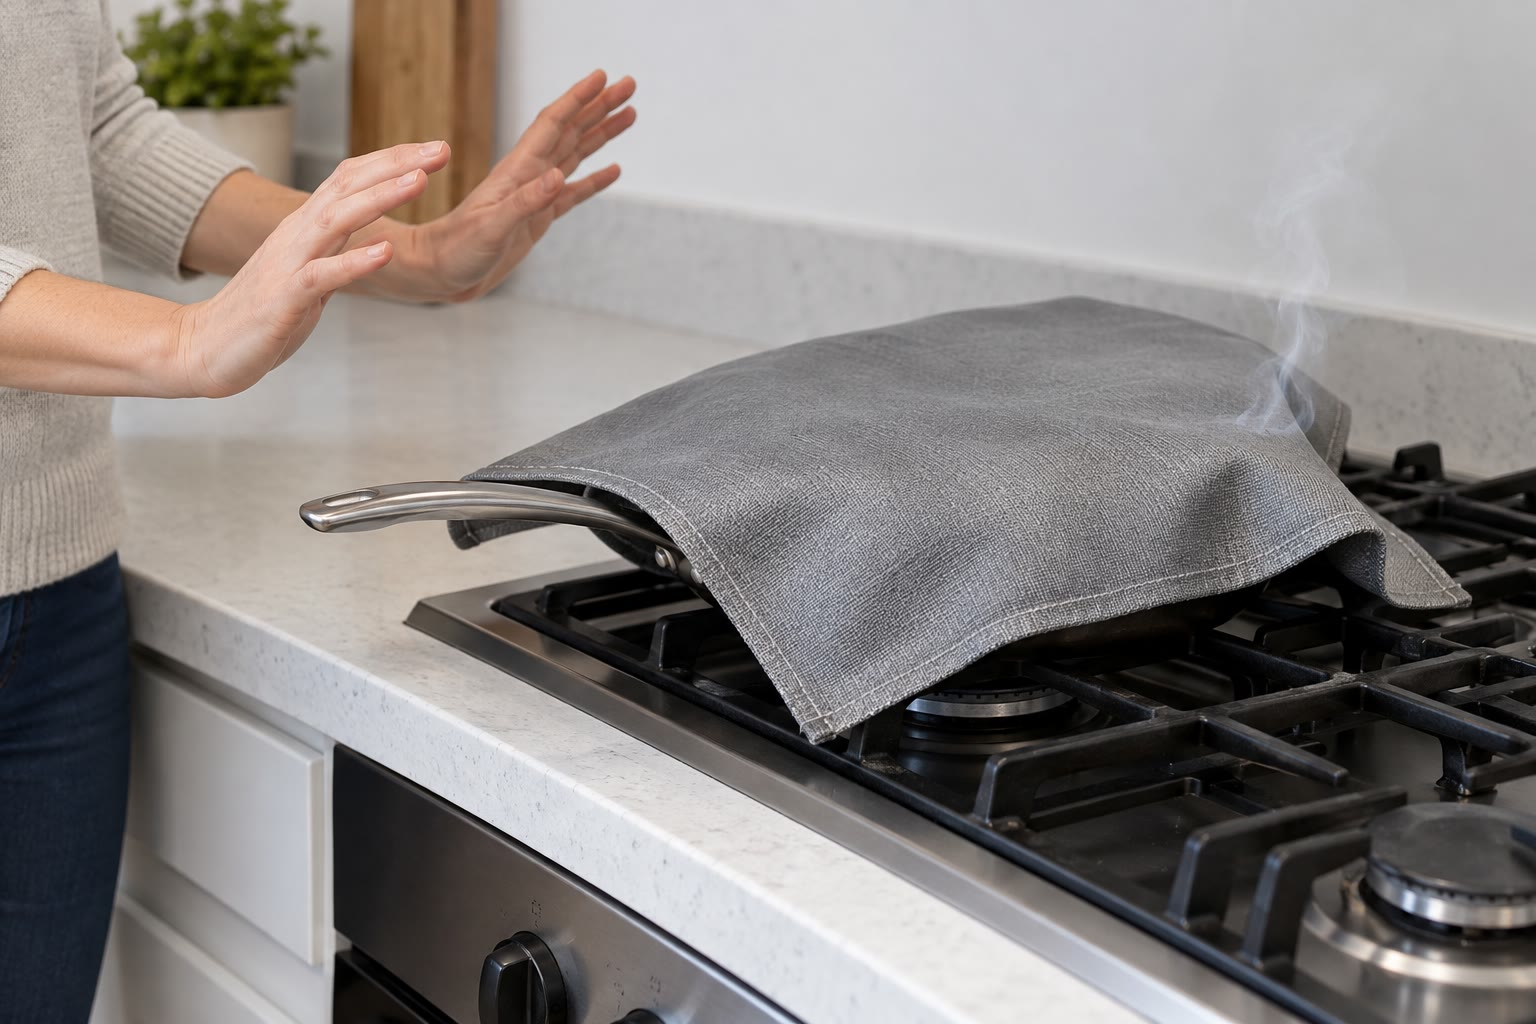
\includegraphics[width=\linewidth,height=4.6cm,keepaspectratio]{images/book1/ai/g4-fire-blanket.jpg}

{\small بطانية إطفاء فوق مقلاة: لم يعد \omterm{def:g4:air-a-mixture-of-gases:air}{الهواء} يصل إلى
النار.}
\end{minipage}\hfill
\begin{minipage}[t]{0.48\linewidth}\centering
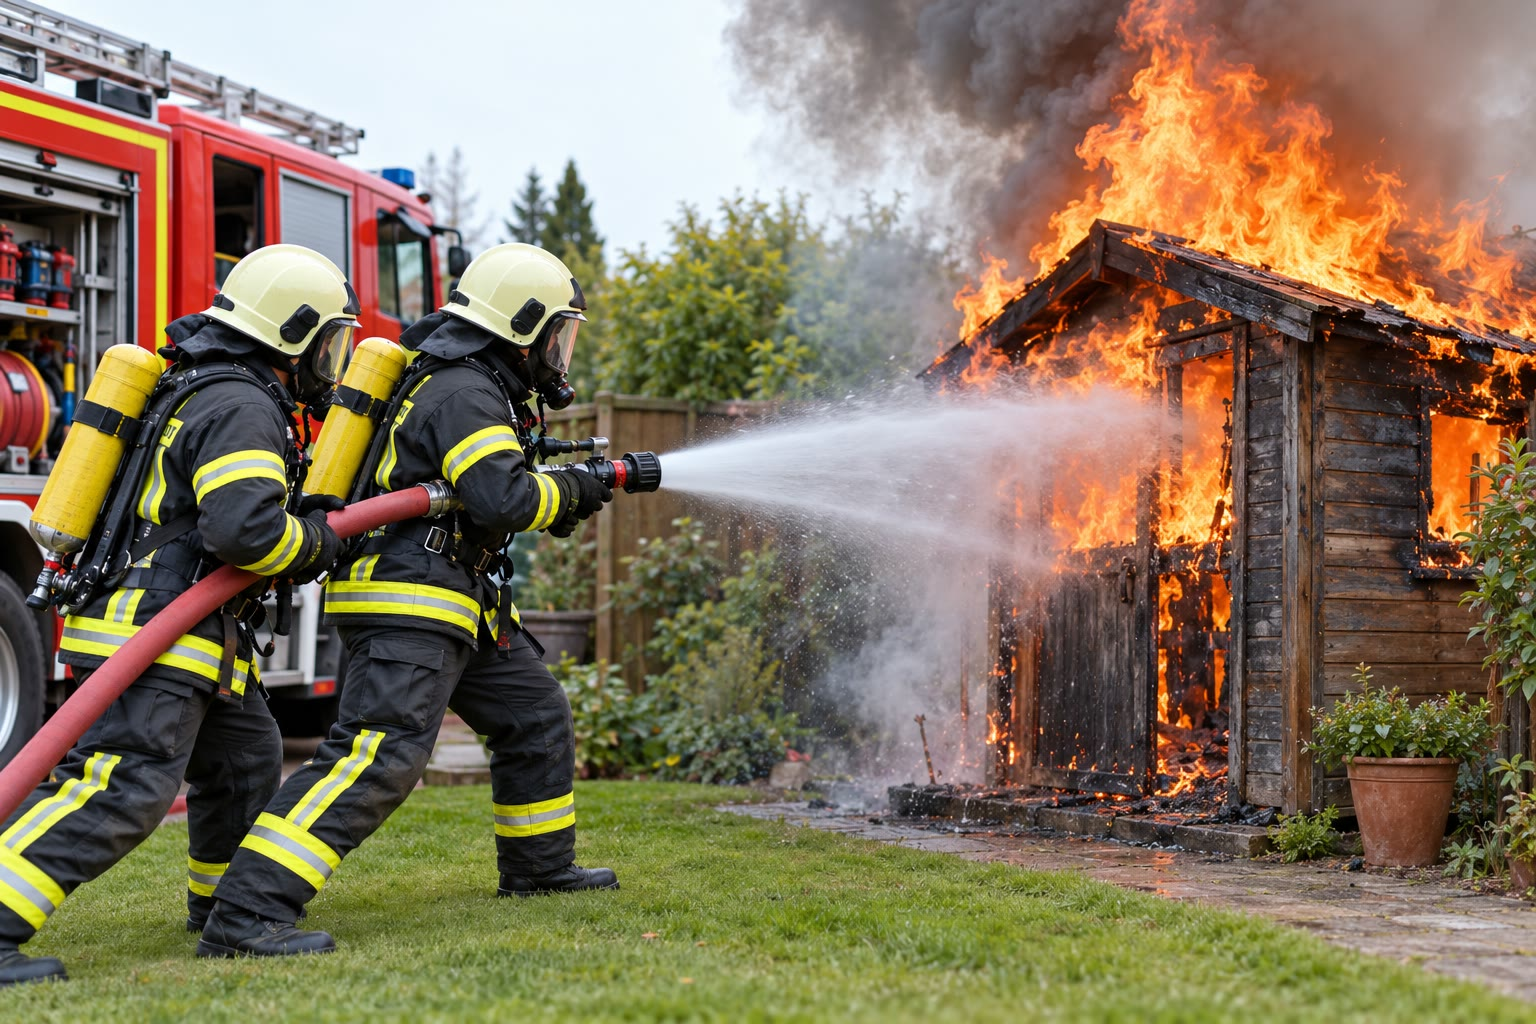
\includegraphics[width=\linewidth,height=4.6cm,keepaspectratio]{images/book1/ai/g4-firefighters.jpg}

{\small رجال الإطفاء يرشّون الماء ليبرّدوا سقيفة تحترق.}
\end{minipage}
\end{omfigure}

\section{السلامة من الحرائق}

\begin{remark}[لا ماء أبدًا على مقلاة زيت مشتعل]\label{rem:g4:what-a-fire-needs:oil}
إذا اشتعل الزيت في مقلاة فلا يجوز لأحد أن يرمي عليه الماء: فالماء يغلي
فورًا تحت الزيت ويقذف الزيت المشتعل خارج المقلاة. بل يُطفئ شخص بالغ
الغاز أو صفيحة الطهي، ويغطي المقلاة بغطاء أو ببطانية إطفاء.
\end{remark}

\begin{safety}{\ghs{GHS02}\ghs{GHS04}}
% ledger: ghs:butane
الغاز الذي في القداحة أو في عبوة التخييم هو البيوتان. ورمز اللهب
(GHS02) يعني: شديد القابلية للاشتعال، يُحفظ بعيدًا عن اللهب
والشرر. ورمز قارورة الغاز (GHS04) يعني: غاز محفوظ تحت
الضغط.
\end{safety}

\begin{proposition}[ماذا تفعل إذا وقع حريق]\label{prop:g4:what-a-fire-needs:safety}
الدخان هو الخطر الأول في الحريق: فهو ساخن، ويحجب طريق الخروج، واستنشاقه
سام. وجهاز إنذار الدخان المثبت في السقف يطلق صفيرًا عاليًا ما إن يصل إليه
الدخان. فإذا وقع حريق: اخرج، وابقَ منخفضًا تحت الدخان، وأغلق الأبواب
خلفك، واتصل برجال الإطفاء من الخارج. ولا تعد إلى الداخل
أبدًا.
\end{proposition}

\begin{omfigure}
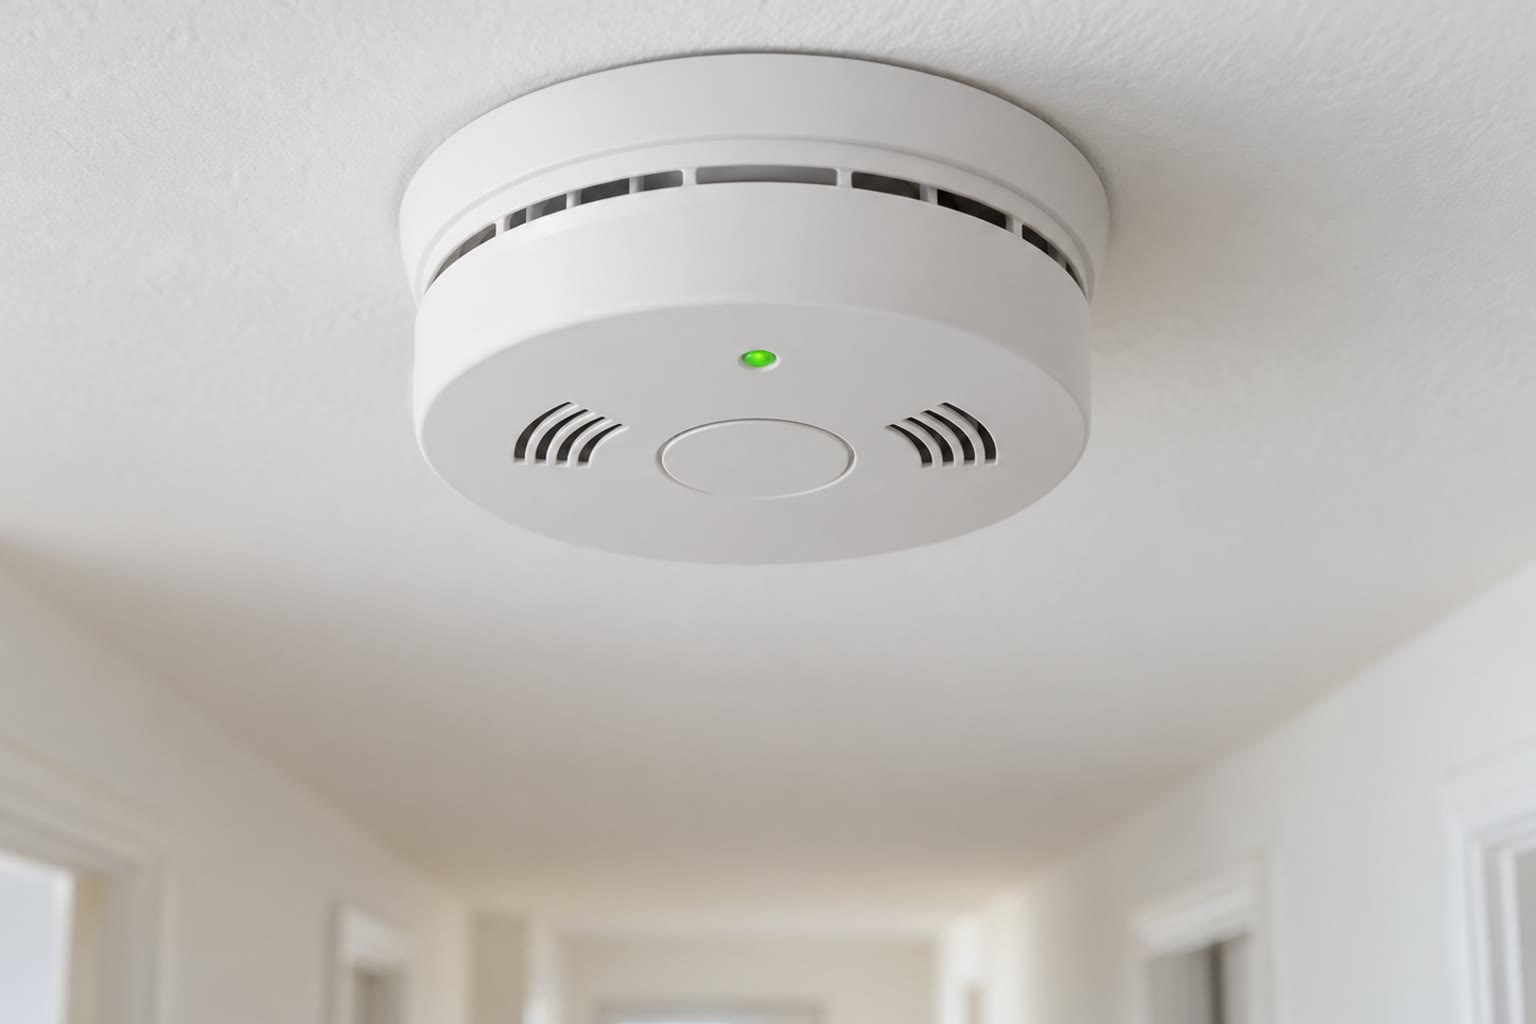
\includegraphics[width=0.42\linewidth]{images/book1/ai/g4-smoke-alarm.jpg}

{\small جهاز إنذار الدخان: يصفر ما إن يصل إليه الدخان.}
\end{omfigure}

\section{تمارين}

\begin{exercise}[$\star$]\label{exo:g4:what-a-fire-needs:1}
سمِّ أضلاع \omterm{def:g4:what-a-fire-needs:fire-triangle}{مثلث النار} الثلاثة.
\end{exercise}

\begin{exercise}[$\star$]\label{exo:g4:what-a-fire-needs:2}
أي هذه المواد \omterm{def:g4:what-a-fire-needs:fuel}{وقود}: الخشب، والرمل، وشمع الشموع، والزجاج، والبنزين،
والماء، والورق؟
\end{exercise}

\begin{exercise}[$\star$]\label{exo:g4:what-a-fire-needs:3}
تُرمى بطانية إطفاء على نار صغيرة. أي ضلع من أضلاع \omterm{def:g4:what-a-fire-needs:fire-triangle}{مثلث النار}
تنزعه؟
\end{exercise}

\begin{exercise}[$\star$]\label{exo:g4:what-a-fire-needs:4}
يرشّ رجال الإطفاء الماء على سقيفة تحترق. أي ضلع من أضلاع \omterm{def:g4:what-a-fire-needs:fire-triangle}{مثلث النار}
ينزعه الماء؟
\end{exercise}

\begin{exercise}[$\star$]\label{exo:g4:what-a-fire-needs:5}
سمِّ ثلاث مواد جديدة تنتج حين يحترق الخشب.
\end{exercise}

\begin{exercise}[$\star$]\label{exo:g4:what-a-fire-needs:6}
لماذا يعود الجمر المتوهج إلى \omterm{def:g4:what-a-fire-needs:burning}{الاشتعال} حين ننفخ عليه؟
\end{exercise}

\begin{exercise}[$\star$]\label{exo:g4:what-a-fire-needs:7}
كأس باردة نمسكها فوق شمعة فتتغشى. ما المادة الجديدة التي صنعتها
الشمعة؟
\end{exercise}

\begin{exercise}[$\star$]\label{exo:g4:what-a-fire-needs:8}
ماذا تفعل أولًا إذا انطلق جهاز إنذار الدخان ورأيت دخانًا؟
\end{exercise}

\begin{exercise}[$\star$]\label{exo:g4:what-a-fire-needs:9}
انظر إلى الشكل الذي فيه المثلثات الثلاثة الصغيرة. أي ضلع يُشطب حين
يُغلق الغاز؟
\end{exercise}

\begin{exercise}[$\star\star$]\label{exo:g4:what-a-fire-needs:10}
لإيقاف حريق غابة يقطع رجال الإطفاء أحيانًا شريطًا عريضًا من الأشجار أمامه.
أي ضلع من أضلاع \omterm{def:g4:what-a-fire-needs:fire-triangle}{مثلث النار}
ينزعون؟
\end{exercise}

\begin{exercise}[$\star\star$]\label{exo:g4:what-a-fire-needs:11}
الحطبة أثقل بكثير من رمادها. هل اختفى جزء من الحطبة؟ اشرح إلى
أين ذهب.
\end{exercise}
